\documentclass{article}

% if you need to pass options to natbib, use, e.g.:
%     \PassOptionsToPackage{numbers, compress}{natbib}
% before loading neurips_2021

% ready for submission

% to compile a preprint version, e.g., for submission to arXiv, add add the
% [preprint] option:
%     \usepackage[preprint]{neurips_2021}

% to compile a camera-ready version, add the [final] option, e.g.:
\usepackage[final]{workshop}

% to avoid loading the natbib package, add option nonatbib:
%    \usepackage[nonatbib]{neurips_2021}

\usepackage{wrapfig}
\usepackage{graphicx}
\usepackage{fontawesome}

\usepackage[utf8]{inputenc} % allow utf-8 input
\usepackage[T1]{fontenc}    % use 8-bit T1 fonts
\usepackage{hyperref}       % hyperlinks
\usepackage{url}            % simple URL typesetting
\usepackage{booktabs}       % professional-quality tables
\usepackage{amsfonts}       % blackboard math symbols
\usepackage{nicefrac}       % compact symbols for 1/2, etc.
\usepackage{microtype}      % microtypography
\usepackage{xcolor}         % colors
\usepackage{tabularx}
\usepackage{array}
\usepackage{multicol}

\usepackage{float}
\usepackage{pgf}
\usepackage{tikz}
\usetikzlibrary{arrows,automata,snakes}
\usepackage{rotating}

\setlength{\columnsep}{0pt}

\usepackage{abstract}
\renewcommand{\abstractname}{}    % clear the title
\renewcommand{\absnamepos}{empty} % originally center


\title{Advances in Programming Languages\\ and Neurosymbolism (AIPLANS II)}

% The \author macro works with any number of authors. There are two commands
% used to separate the names and addresses of multiple authors: \And and \AND.
%
% Using \And between authors leaves it to LaTeX to determine where to break the
% lines. Using \AND forces a line break at that point. So, if LaTeX puts 3 of 4
% authors names on the first line, and the last on the second line, try using
% \AND instead of \And before the third author name.

\author{%
  Jialu Bao$^3$, Maddy Bowers$^2$, Breandan Considine$^{1, 10}$, \\\textbf{Younesse Kaddar$^{5, 11}$, Justine Gehring$^{9, 12}$, Shawn Tan$^{4, 10}$} \\
%    \texttt{\{considib, shrivast, huidavid, tanjings\}@mila.quebec} \\
    David Chiang$^6$, Parisa Kordjamshidi$^$, Nikolay Malkin$^9$, Xujie Si$^{8, 12}$\\\\
    McGill$^1$, MIT$^2$, Cornell$^3$, Universit\'e de Montr\'eal$^4$, Oxford$^{5}$, Notre Dame$^6$,\\University of Toronto$^7$, Michigan State University$^8$, University of Edinburgh$^9$,\\Mila$^{10}$, Cohere$^{11}$, Moderne$^{12}$, Vector$^{13}$
}

\begin{document}

    \maketitle
    \vspace{-0.5cm}
    \begin{abstract}
        % A very brief advertisement or tagline for the workshop, up to 140 characters, that highlights any key information you wish prospective attendees to know, and which would be suitable to be put onto a web-based survey (see below).
        \textbf{Tagline:} AIPLANS: Fusing machine learning with programming language theory to create neurosymbolic programming machines! \url{https://aiplans.github.io} % Are you curious whether machines can write programs that are both sound and interpretable? Come check out AIPLANS, a new workshop on domain-specific languages for learning and synthetic reasoning, to be hosted at NeurIPS 2021!
    \end{abstract}

   Since the first AIPLANS workshop at NeurIPS 2021, rapid progress has been made on uniting the two divergent branches of computer science: machine learning (ML) and programming languages (PL). What was once a fringe research area has begun to catalyze a broader movement, with summer schools~\cite{munawar2023neurosymbolic, costilla2024neurosymbolic}, workshops~\cite{besold2023nesy, belle2023neurosys, munawar2024neurosymbolic, llievski2024neurosymbolic} and tutorials~\cite{palangi2022tutorial, chaudhuri2023poplneurosym, shakarian2024tutorial} dedicated to neurosymbolic research in recent years. From the connectionists, descended the present generation of large langauge models, inspired by biological systems and immersed in probability, statistics and linear algebra. And from the symbolists came programming languages, compilers, and automated theorem provers, powering the digital revolution which made this endevor even possible.

%    Machine learning, though powerful, is generally concerned with naturalness, generalization and scalability, while programming languages care much more deeply about soundness, completeness and interpretability.

    AIPLANS seeks to harness the emergent capabilities of large language models to the explainability and rigor of the symbolic method, taking inspiration from the experimentalist, language designer, programming enthusiast, and formalist alike. But how do we build systems with the prowess of large language models while retaining the safety and trustworthiness of programming langauges? Can we make them flexible enough to behave naturally while simple enough to be interpretable? And how do we guaratnee these systems plan and act safely amidst humans? At AIPLANS, we aim to explore these questions with an eye towards \textit{program synthesis} -- human-readable and mechanically verifiable specifications that can be interpreted by a computer. In a series of invited talks, contributed papers, and panel discussions, we plan to cover some of the following areas:

    \begin{multicols}{2}
     \begin{itemize}
        \item Probabilistic model checking
        \item Language induction
        \item Proof search and program synthesis
        \item Declarative programming
        \item Constraint satisfaction
        \item Unification, completion and resolution
        \item Analytic combinatorics
        \item Computational group theory
        \item Vector symbolic architectures
        \item Automata and formal grammars
        \item Formal aspects of language modeling~\cite{cotterell2023formal}
        \item Constrained sampling from LLMs
        \item Randomized complexity
        \item Algorithmic information theory
        \item Circuit lower bounds
        \item Reachability problems
        \item Proof assistance and automation
        \item Type theory and semantics
    \end{itemize}
    \end{multicols}

    \clearpage

    % \begin{figure}[H] %Remove this if low on space
    %     \centering
    %     \begin{tikzpicture}[->,>=stealth',shorten >=1pt,auto,node distance=2.8cm, semithick]
    %         % \tikzstyle{every state}=[draw=none,text=white]

    %         \node[state]         (A)                    {PL};
    %         \node[state]         (B) [right of=A]       {ML};

    %         \path (A) edge [bend left] node {ADs, PPLs, DSLs} (B)
    %         (B) edge [bend left] node {Ideas, features, tools} (A);
    %     \end{tikzpicture}
    %     \caption{The virtuous cycle of machine learning and programming languages research.}
    % \end{figure}

    % Applying techniques from programmable inference to transform and generate programs, and adapting insights gained developing those programs to drive innovation in higher-order AD and probabilistic programming is a virtuous cycle. As researchers grow more accustomed to outsourcing low-level reasoning tasks to automatic programming systems, we anticipate cooperation between automatic and synthetic programming will continue to increase.  A joint workshop such as the one put forward in this proposal could help to facilitate yet-unrealized research connections among neighboring fields.
    %%%%%%%%%%%%%%%%%%%%%%%%%%%%%%%%%%%%%%%%%%%%%%%%%%


    % Much work remains.
    % Similar domain-specific languages have shown progress automating inference in other logical disciplines, such as belief nets, proof nets, and related message passing schemes on tree- and graph-structured data.

    % Similarly, the programming language community too, has its blind spots. PL could take a page from structured inference and propagation algorithms as a medium for distributed computation.

    % In exchange, we believe a great deal of progress can be achieved, in particular, between automatic and synthetic programming. For illustration, we include the following incomplete list of topics:

    % \begin{itemize}
    % \item Differentiable programming / algorithmic differentiation
    % \item Probabilistic programming / statistical inference
    % \item Dynamic programming / reinforcement learning
    % \item Program induction / program synthesis
    % \item Functional programming / $\lambda$-calculus
    % \item Semiring programming / message passing
    % \item Array programming / linear algebra
    % \item Meta-programming / meta-learning
    % \item Logic programming / Relational programming
    % \end{itemize}





    \section*{Proposed Workshop Logistics}

    % A description of special requirements and technical needs.
    AIPLANS will be a one-day in-person workshop with live talks and panels. Talks will be hosted in English, following the standard format of oral presentations and panel discussions, to be concluded with a poster session. Proceedings will be non-archival. Outside of standard videoconferencing and SlidesLive assistance, no other technical requirements are necessary. We anticipate receiving roughly 200 participants, including speakers and workshop submitters, based on our experience running AIPLANS at NeurIPS 2021 and attendance at similarly-themed workshops in prior years.

%    . A partial list of speakers who have confirmed their presence (pending workshop acceptance) follows:
%
%    \begin{center}
%        \begin{tabular}{ c c c }
%            \href{https://www.cse.msu.edu/~kordjams/}{Parisa Kordjamshidi}
%        \end{tabular}
%    \end{center}

    % A list of invited speakers, if applicable, with an indication of which ones have already agreed and which are indicative.
    % We plan to invite four keynote speakers.  Three system developers, and one programming language theoretician.  TODO:
    % \begin{itemize}
    %     \item
    % \end{itemize}

    The workshop itself will run for approximately eight hours, featuring four 45-minute contributed talks and up to six 20-minute contributed talks, with a strong preference for in-person attendance. AIPLANS will solicit four-page paper submissions in a CFP to be circulated pending workshop acceptance. To encourage submissions from the broader ML/PL community, accepted authors will be given an opportunity to showcase their work in a poster session, and exceptional contributions may be selected for a short spotlight talk. We expect to receive 30-40 submissions, and pledge that each paper will receive at least two fair and independent reviews. To minimize potential conflicts of interest, AIPLANS will manage submissions via \href{https://openreview.net}{OpenReview}.

    % An account of the efforts made to ensure diversity of the organizers and speakers (WiML, Black in AI, and LXAI directories, among others, may be a useful resource). Also an account of any efforts to include diverse participants (e.g., via mentoring, subsidies, or the wording and topics in the CFP).

    Those who traditionally publish in venues such as SIGPLAN, SIGSOFT and other ACM venues are encouraged to submit work they consider relevant to a machine learning audience, provided that effort is taken to ensure its accessibility. Special consideration will be given to pedagogical submissions of outstanding clarity. Further information, including evaluation criteria, examples of relevant literature, deadlines and workshop logistics will be provided for reference.

    %   By submitting a workshop proposal, workshop organizers commit to notifying those who submit contributions (including talks and posters) to the workshop of their acceptance status before Oct 22, 2021. A timeline should be included in the proposal that will allow for this.

    \begin{figure}[H]
        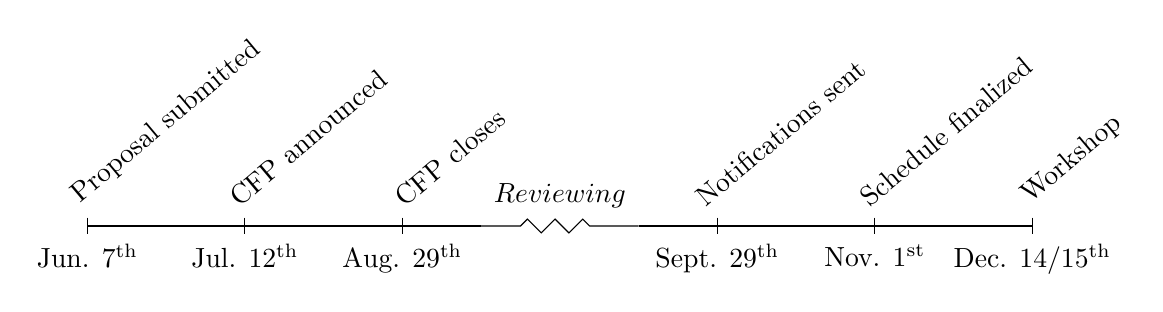
\begin{tikzpicture}[snake=zigzag, line before snake = 5mm, line after snake = 5mm]
            % draw horizontal line
            \draw (0,0) -- (5,0);
            \draw[snake] (5,0) -- (7,0);
            \draw (7,0) -- (12,0);


            % draw vertical lines
            \foreach \x in {0, 2, 4, 8, 10, 12}
            \draw (\x cm,3pt) -- (\x cm,-3pt);

            % draw nodes

            \draw (0,0) node[below=3pt] {Jun. 7\textsuperscript{th}} node[above=3pt] {};
            \draw (1,0) node[below=3pt] {} node[above=3pt] {$\begin{turn}{40}  Proposal submitted \end{turn} $};
            \draw (2,0) node[below=3pt] {Jul. 12\textsuperscript{th}} node[above=3pt] {};

            \draw (2.8,0) node[below=3pt] {} node[above=3pt] {$\begin{turn}{40}  CFP announced \end{turn} $};
            \draw (4,0) node[below=3pt] {Aug. 29\textsuperscript{th}} node[above=3pt] {};
            \draw (4.6,0) node[below=3pt] {} node[above=3pt] {$\begin{turn}{40}  CFP closes \end{turn} $};
            \draw (6,0) node[below=3pt] {} node[above=3pt] {$ Reviewing $};
            \draw (8,0) node[below=3pt] {Sept. 29\textsuperscript{th}} node[above=3pt] {};
            \draw (8.8,0) node[below=3pt] {} node[above=3pt] {$\begin{turn}{40}  Notifications sent \end{turn} $};
            \draw (10,0) node[below=3pt] {Nov. 1\textsuperscript{st}} node[above=3pt] {};
            \draw (10.9,0) node[below=3pt] {} node[above=3pt] {$\begin{turn}{40}  Schedule finalized \end{turn} $};
            \draw (12,0) node[below=3pt] {Dec. 14/15\textsuperscript{th}} node[above=3pt] {};
            \draw (12.5,0) node[below=3pt] {} node[above=3pt] {$\begin{turn}{40} Workshop \end{turn} $};
        \end{tikzpicture}
        \caption{A tentative timeline for our proposed workshop at NeurIPS 2024.}
    \end{figure}

    If accepted, AIPLANS will announce its CFP and pursue contributions from the broader ML/PL community shortly thereafter. Six weeks later, the CFP will close on Aug. 29\textsuperscript{th}. This deadline may be extended to no later than Sept. 5\textsuperscript{th}, depending on the volume of submissions received, leaving sufficient time for referees and program chairs to give feedback. Authors will be notified of acceptance no later than Sept. 29\textsuperscript{th}. We intend to finalize the schedule and coordinate presentation logistics between Nov. 1\textsuperscript{st} and Dec. 14\textsuperscript{th}. Those who wish to prerecord talks will be given an opportunity to do so. The final workshop will consist of prerecorded and live talks with Q\&A, followed by a moderated panel, and poster session. Further details about schedule and logistics will be made available, pending acceptance at: \url{https://aiplans.github.io}.

    AIPLANS is an equal-opportunity workshop that celebrates cultural, linguistic, ethnic and intellectual diversity in all forms. Not only are we committed to nondiscrimination on the basis of, e.g., race, creed, age, gender, orientation, physical or mental handicap, but also aim to encourage individuals from other disadvantaged and underrepresented socioeconomic backgrounds to participate. Should our workshop be accepted, scholarships covering the cost of registration will be extended for those who wish to attend but would otherwise be unable to do so due to financial hardship. If needed, AIPLANS may pursue industry sponsorship for this initiative to enable a wider audience to attend. Further details about registration and funding availability will be provided in a timely manner.


    \newpage


    \section*{Confirmed Workshop Organizers}\vspace{-0.5cm}
    \begin{table}[h!]
        \begin{center}
            \begin{tabular}{ c p{10.5cm}}

                \raisebox{-\totalheight}{\includegraphics[width=0.16\textwidth]{../img/organizers/jialu}} & \vspace*{0.2cm}\textbf{Jialu Bao} is a Ph.D. student at Cornell advised by Prof. Justin Hsu, who is working on the verification of randomized algorithms. Before moving to Cornell with her advisor, she spent two years at University of Wisconsin – Madison as a Ph.D. student, and prior to that, did her undergrad at Cornell majoring in Mathematics and Computer Science. \vspace*{0.1cm}\newline\faHome \,\url{https://baojia.lu} \faTwitter \href{https://twitter.com/howowhy}{ @howowhy}\\\\\\

                \raisebox{-\totalheight}{\includegraphics[width=0.16\textwidth]{../img/organizers/maddy}} & \textbf{Maddy Bowers} is a Ph.D. student at MIT, co-advised by Armando Solar-Lezama in EECS and Josh Tenenbaum in BCS, whose research combines methods from programming languages (PL) research with machine learning to tackle problems in artificial intelligence. \vspace*{0.1cm}\newline\faHome \,\url{https://mlb2251.github.io/} \faTwitter \href{https://x.com/mattlbowers}{ @mattlbowers}\\\\\\

                \raisebox{-\totalheight}{
\includegraphics[width=0.16\textwidth]{../img/organizers/breandan}} & \textbf{Breandan Considine} is a Ph.D. student at McGill University co-supervised by Jin Guo and Xujie Si. His research studies how to reason about the behavior of real-world programs and build more intelligent programming tools for developers. Previously, he organized the first \href{https://aiplans.github.io/}{AIPLANS} workshop at NeurIPS and co-organized the ICLR workshop, \href{https://rethinkingmlpapers.github.io/}{Rethinking ML Papers}. \vspace*{0.1cm}\newline \faHome \,\url{https://breandan.github.io} \faTwitter \href{https://x.com/breandan}{ @breandan} \\\\\\

                \raisebox{-\totalheight}{\includegraphics[width=0.16\textwidth]{../img/organizers/younesse}} & \textbf{Younesse Kaddar} is a Ph.D. student in theoretical computer science at the University of Oxford, working on programming language semantics, Bayesian probabilistic programming, and category theory. Previously, he was a visiting researcher at Mila, Qu\'ebec working with Yoshua Bengio.\vspace*{0.1cm}\newline\faHome \,\url{https://younesse.net/} \faTwitter \href{https://twitter.com/you_kad}{ @you\_kad}\\\\\\

                \raisebox{-\totalheight}{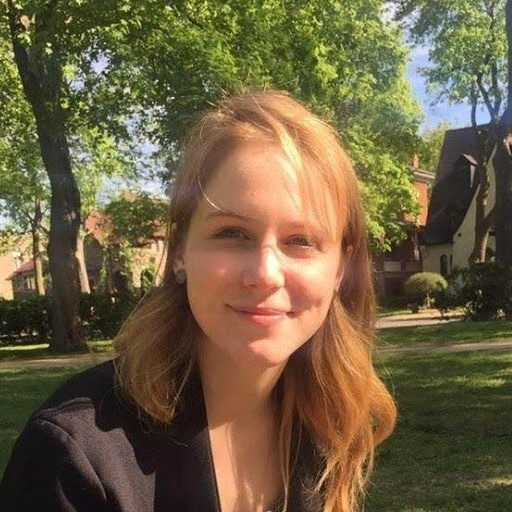
\includegraphics[width=0.16\textwidth]{../img/organizers/justine}} & \vspace*{0.4cm}\textbf{Justine Gehring} is a research engineer at Moderne working in the field of Machine Learning (ML) for code and Graph Neural Networks (GNNs). Her focus lies in generating code under challenging circumstances, specifically in scenarios such as sparse data where library-specific code is required, as well as managing a substantial amount of code at a time. She completed her Master’s Degree in Computer Science at Mila \& McGill. \vspace*{0.1cm}\newline \faHome \,\url{https://justine-gehring.github.io/} \faTwitter \href{https://x.com/GehringJustine}{ @GehringJustine}\\\\\\

                \raisebox{-\totalheight}{
\includegraphics[width=0.16\textwidth]{../img/organizers/shawn}} & \vspace*{0.4cm}\textbf{Shawn Tan} is a Ph.D. candidate at Mila, Universit\'e de Montr\'eal. He is interested in differentiable methods for structured prediction, specifically in the domain of natural language. He co-authored the \href{https://arxiv.org/abs/1810.09536}{Ordered Neurons} paper which won best paper at ICLR 2019. \vspace*{0.1cm}\newline \faHome \,\url{http://blog.wtf.sg} \faTwitter \href{https://twitter.com/tanshawn}{ @tanshawn}\\\\\\
            \end{tabular}
        \end{center}
    \end{table}


    \pagebreak

    \section*{Confirmed Program Committee}

    \vspace*{-0.23cm}\begin{table}[h!]
        \begin{center}
            \begin{tabular}{ c p{10.5cm}}
                \raisebox{-\totalheight}{
\includegraphics[width=0.16\textwidth]{../img/chairs/david}} & \textbf{David Chiang} is a Professor at Notre Dame University. His research is in natural language processing, the subfield of computer science that aims to enable computers to understand and produce human language. He focuses mainly on language translation, and has interests in syntactic parsing and other areas as well. \vspace*{0.1cm}\newline \faHome \,\url{https://www3.nd.edu/~dchiang/} \faTwitter \href{https://x.com/davidweichiang}{ @davidweichiang} \\\\\\

                \raisebox{-\totalheight}{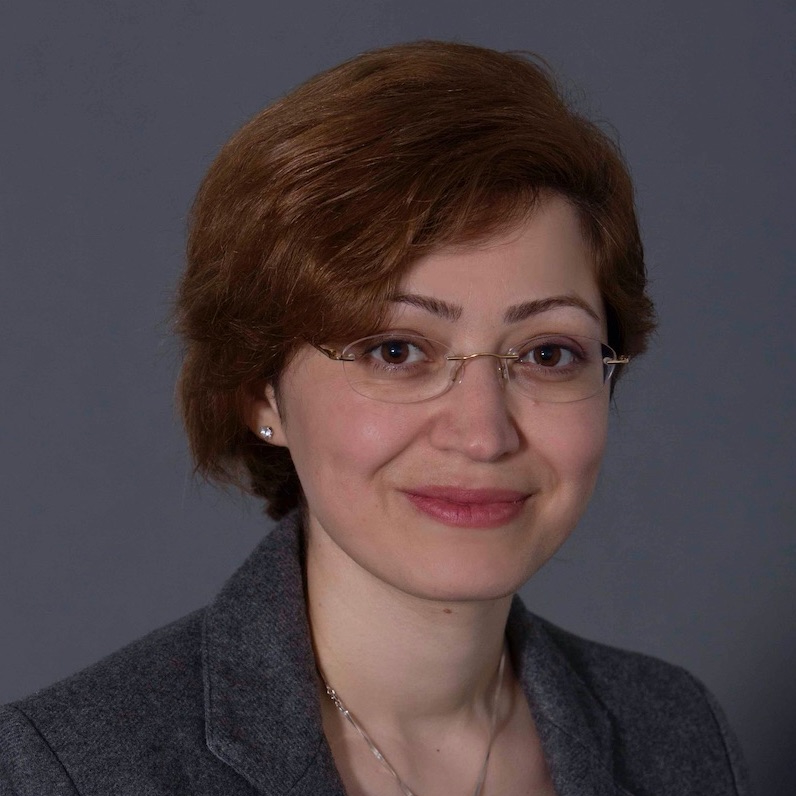
\includegraphics[width=0.16\textwidth]{../img/chairs/parisa}} & \textbf{Parisa Kordjamshidi} is an assistant professor at Michigan State University and director of the Heterogeneous Learning and Reasoning (HLR) lab. Her main research interests are artificial intelligence, machine learning, natural language processing, and declarative learning based programming (DeLBP). She works on the extraction of formal semantics and structured representations from natural language, with a specific focus on spatial semantics representation and structured output learning models. \vspace*{0.1cm}\newline \faHome \,\url{https://www.cse.msu.edu/~kordjams/} \faTwitter \href{https://x.com/Kordjamshidi}{ @Kordjamshidi} \\\\\\

                \raisebox{-\totalheight}{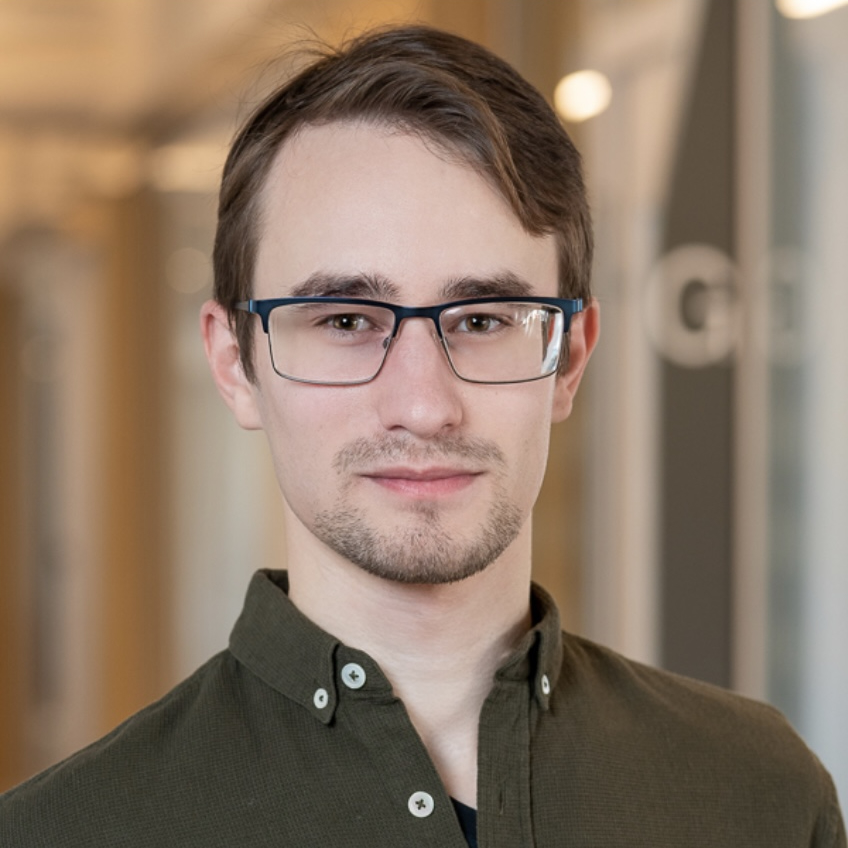
\includegraphics[width=0.16\textwidth]{../img/chairs/kolya}} & \textbf{Nikolay Malkin} is an Associate Professor at the University of Edinburgh working on algorithms for deep-learning-based reasoning and their applications, in particular  induction of compositional structure in generative models, modeling of posteriors over high-dimensional explanatory variables, uncertainty-aware explanations for observed data, human-like symbolic, formal, and mathematical reasoning and tracking land use patterns over time and monitoring the effects of climate change. \vspace*{0.1cm}\newline \faHome \,\url{https://malkin1729.github.io/} \\\\\\

                \raisebox{-\totalheight}{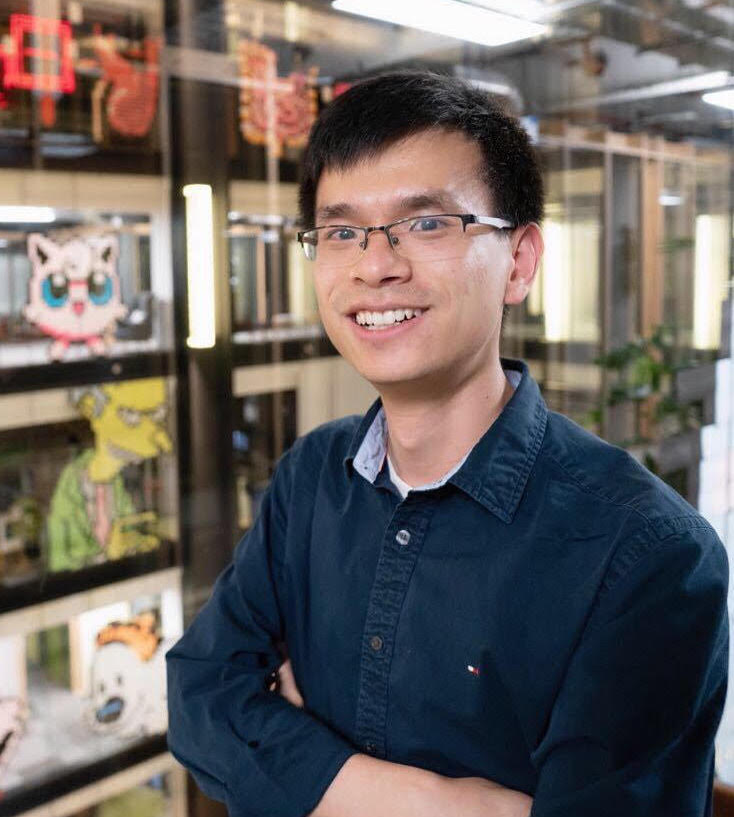
\includegraphics[width=0.16\textwidth]{../img/chairs/xujie}} &\textbf{Xujie Si} is an Assistant Professor and Canada CIFAR AI Chair in the School of Computer Science at the University of Toronto and Vector Institute. He finished his Ph.D. in Computer and Information Science at the University of Pennsylvania in 2020, advised by Prof. Mayur Naik. Xujie received his M.S. in computer science from Vanderbilt University in 2014, before which he obtained his B.E. (with Honors) from Nankai Unversity in 2011. \vspace*{0.1cm}\newline \faHome  \,\url{https://www.cs.mcgill.ca/~xsi} \faTwitter \href{https://twitter.com/xujiesi}{ @XujieSi} \\\\\\

%                \raisebox{-\totalheight}{
\includegraphics[width=0.16\textwidth]{../img/chairs/danny}} & \textbf{Danny Tarlow} is a Research Scientist at the Google Brain team in Montreal. He is primarily interested in machine learning methods for understanding and generating programs, but has broad interests across Machine Learning. Danny is also an Adjunct Professor in the School of Computer Science at McGill University and an associate member at Mila, where he co-supervises a couple PhD students. He holds a PhD from the Machine Learning group at University of Toronto (2013) and before coming to Montreal, spent four years as a postdoc and then researcher at Microsoft Research, Cambridge. \vspace*{0.1cm}\newline \faHome \, \url{https://research.google/people/DannyTarlow} \faTwitter \href{https://twitter.com/dtarlow2}{ @dtarlow2} \\\\\\

%                \raisebox{-\totalheight}{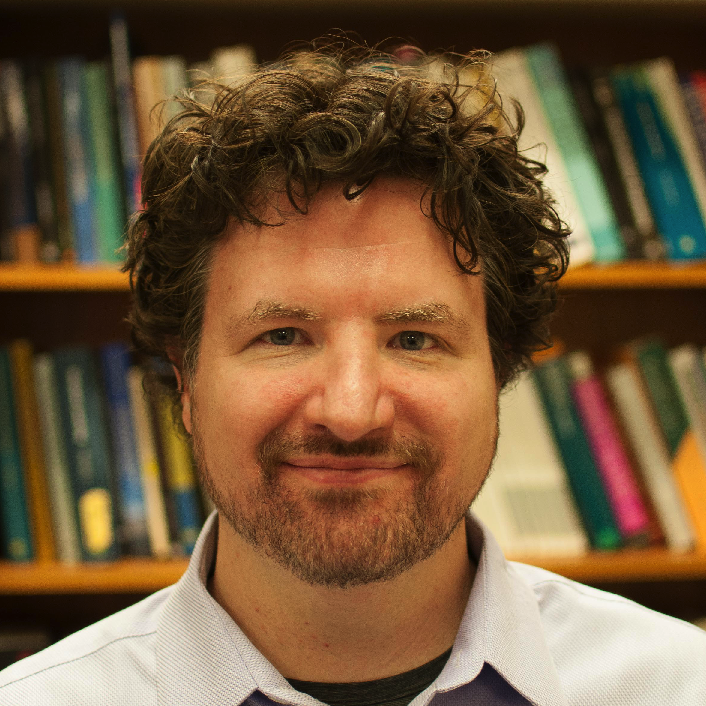
\includegraphics[width=0.16\textwidth]{../img/chairs/tim}} & \vspace*{0.2cm}\textbf{Timothy O'Donnell} is an Assistant Professor in the Department of Linguistics at McGill University developing mathematical models of language generalization, learning, and processing. His research draws on experimental methods from psychology, formal modeling techniques from NLP, theoretical tools from linguistics, and problems from all three. \vspace*{0.1cm}\newline \faHome \, \url{http://people.linguistics.mcgill.ca/~timothy.odonnell/} \\\\\\
            \end{tabular}
        \end{center}\label{tab:table}
    \end{table}

    \clearpage
    \bibliography{workshop}
    \bibliographystyle{plain}

\end{document}